\documentclass[notitlepage]{report}
\usepackage{layout}
\usepackage[a4paper, total={5in,9in}]{geometry}
\usepackage[T1]{fontenc}
\usepackage{mathtools}
\usepackage{amsthm}
\usepackage[framemethod=TikZ]{mdframed}
\usepackage{amsmath}
\usepackage{amssymb}
\usepackage{cancel}
\usepackage[dvipsnames]{xcolor}
\usepackage{tikz}
\usepackage{tikz-cd}
\usepackage{pgfplots}
\pgfplotsset{compat=1.18}
\usepackage[many]{tcolorbox}
\usepackage{import}
\usepackage{pdfpages}
\usepackage{transparent}
\usepackage{enumitem}
\usepackage[colorlinks]{hyperref}
\usepackage{csvsimple}
\usepackage{listings}
\usepackage{booktabs}
\usepackage{graphicx}
\usepackage{subcaption}

\newcommand*{\sminus}{\raisebox{1.3pt}{$\smallsetminus$}}

\newcommand*{\transp}[2][-3mu]{\ensuremath{\mskip1mu\prescript{\smash{\mathrm t\mkern#1}}{}{\mathstrut#2}}}%

% newcommand for span with langle and rangle around
\newcommand{\Span}[1]{{\left\langle#1\right\rangle}}

\newcommand{\incfig}[2][1]{%
    \def\svgwidth{#1\columnwidth}
    \import{./figures/}{#2.pdf_tex}
}

\pdfsuppresswarningpagegroup=1

\newcounter{theo}[section]\setcounter{theo}{0}
\renewcommand{\thetheo}{\arabic{section}.\arabic{theo}}

\newcounter{excounter}[section]\setcounter{excounter}{0}
\renewcommand{\theexcounter}{\arabic{section}.\arabic{excounter}}

\numberwithin{equation}{section}

\newenvironment{theorem}[1][]{
    \refstepcounter{theo}
     \ifstrempty{#1}
    {\mdfsetup{
        frametitle={
            \tikz[baseline= (current bounding box.east),outer sep=0pt]
            \node[anchor=east,rectangle,fill=blue!20,rounded corners=5pt]
            {\strut~Teorema~\thetheo};}
        }
    }{\mdfsetup{
        frametitle={
            \tikz[baseline= (current bounding box.east),outer sep=0pt]
            \node[anchor=east,rectangle,fill=blue!20,rounded corners=5pt]
            {\strut~Teorema~\thetheo:~#1};}
        }
    }
    \mdfsetup{
        roundcorner=10pt,
        innertopmargin=10pt,linecolor=blue!20,
        linewidth=2pt,topline=true,
        frametitleaboveskip=\dimexpr-\ht\strutbox\relax,
        % nobreak=false
    }
\begin{mdframed}[]\relax}{
\end{mdframed}}
\newtcolorbox[auto counter, number within=section]{definition}[2][]{
    colframe=violet!0,
    coltitle=violet, % Title text color
    fonttitle=\bfseries, % Title font
    title={Definizione~\thetcbcounter:~#2}, % Title format
    sharp corners, % Less rounded corners
    boxrule=0pt, % Line width of the box frame
    toptitle=1mm, % Distance from top to title
    bottomtitle=1mm, % Distance from title to box content
    colbacktitle=violet!5, % Background color of the title bar
    left=0mm, right=0mm, top=1mm, bottom=1mm, % Padding around content
    enhanced, % Enable advanced options
    before skip=10pt, % Space before the box
    after skip=10pt, % Space after the box
    breakable, % Allow box to split across pages
    colback=violet!0,
    borderline west={2pt}{-5pt}{violet!40},
    #1
}

\newenvironment{lemmao}[1][]{
    \refstepcounter{theo}
     \ifstrempty{#1}
    {\mdfsetup{
        frametitle={
            \tikz[baseline= (current bounding box.east),outer sep=0pt]
            \node[anchor=east,rectangle,fill=green!20,rounded corners=5pt]
            {\strut~Lemma~\thetheo};}
        }
    }{\mdfsetup{
        frametitle={
            \tikz[baseline= (current bounding box.east),outer sep=0pt]
            \node[anchor=east,rectangle,fill=green!20,rounded corners=5pt]
            {\strut~Lemma~\thetheo:~#1};}
        }
    }
    \mdfsetup{
        roundcorner=10pt,
        innertopmargin=10pt,linecolor=green!20,
        linewidth=2pt,topline=true,
        frametitleaboveskip=\dimexpr-\ht\strutbox\relax,
        % nobreak=true
    }
\begin{mdframed}[]\relax}{
\end{mdframed}}

\theoremstyle{plain}
\newtheorem{lemma}[theo]{Lemma}
\newtheorem{corollary}{Corollario}[theo]
\newtheorem{proposition}[theo]{Proposizione}

\theoremstyle{definition}
\newtheorem{example}[excounter]{Esempio}

\theoremstyle{remark}
\newtheorem*{note}{Nota}
\newtheorem*{remark}{Osservazione}

\newtcolorbox{notebox}{
  colback=gray!10,
  colframe=black,
  arc=5pt,
  boxrule=1pt,
  left=15pt,
  right=15pt,
  top=15pt,
  bottom=15pt,
}

\DeclareRobustCommand{\rchi}{{\mathpalette\irchi\relax}} % beautiful chi
\newcommand{\irchi}[2]{\raisebox{\depth}{$#1\chi$}} % inner command, used by \rchi
\newtcolorbox[auto counter, number within=section]{eser}[1][]{
    colframe=black!0,
    coltitle=black!70, % Title text color
    fonttitle=\bfseries\sffamily, % Title font
    title={Esercizio~\thetcbcounter~#1}, % Title format
    sharp corners, % Less rounded corners
    boxrule=0pt, % Line width of the box frame
    toptitle=1mm, % Distance from top to title
    bottomtitle=1mm, % Distance from title to box content
    colbacktitle=black!5, % Background color of the title bar
    left=0mm, right=0mm, top=1mm, bottom=1mm, % Padding around content
    enhanced, % Enable advanced options
    before skip=10pt, % Space before the box
    after skip=10pt, % Space after the box
    breakable, % Allow box to split across pages
    colback=black!0,
    borderline west={1pt}{-5pt}{black!70},
}
\newcommand{\seminorm}[1]{\left\lvert\hspace{-1 pt}\left\lvert\hspace{-1 pt}\left\lvert#1\right\lvert\hspace{-1 pt}\right\lvert\hspace{-1 pt}\right\lvert}

\definecolor{codegreen}{rgb}{0,0.6,0}
\definecolor{codegray}{rgb}{0.5,0.5,0.5}
\definecolor{codepurple}{rgb}{0.58,0,0.82}
\definecolor{backcolour}{rgb}{0.95,0.95,0.92}
\lstdefinestyle{mystyle}{
    backgroundcolor=\color{backcolour},   
    commentstyle=\color{codegreen},
    keywordstyle=\color{magenta},
    numberstyle=\tiny\color{codegray},
    stringstyle=\color{codepurple},
    basicstyle=\ttfamily\footnotesize,
    breakatwhitespace=false,         
    breaklines=true,                 
    captionpos=b,                    
    keepspaces=true,                 
    numbers=left,                    
    numbersep=5pt,                  
    showspaces=false,                
    showstringspaces=false,
    showtabs=false,                  
    tabsize=2
}

\lstset{style=mystyle}

\title{Report Lab 3\\\small Experimental Physics for AI 2}
\author{G, D, O}
\date{First semester 2024 \-- 2025}

\begin{document}

\maketitle

\begin{abstract}
    This laboratory experience consisted of three different experiments
    concerning electromagnetism. The first one is a visualization of the
    electric field lines through a conductor. The second one is a measurement of
    earth's magnetic field using the phone's magnetometer. The third one is a
    measurement of the magnetic field induced by a coil.
\end{abstract}


\chapter{Visualization of Electric Potential and Electric Field}

\section{Goal}
The main goal of this experiment is to visualize the field lines of the electric
field inside a conductor. While we can't directly observe the electric field, we
can measure the electric potential at different points inside the conductor and
thus infer the electric field lines, as we know that
\[
    \vec{E} = -\nabla V
\]
Thus what we want to do at first is to measure accurately the electric potential
in a grid of points inside the conductor.

We expect to see that the vector field is mostly aligned vertically inside the
conductor while on the edges it should be slightly more curved due to the lack
of charges on the outside of the conductor, the result is a rectangle with
rounded shapes on the east and west sides.
\section{Method}
Firstly, the chosen conductor is a graphite sheet placed on a flat wooden board,
with a grid of points marked on it.
It has the north and south sides connected with a metal bar. A low current, 5V
DC power supply is connected to the conductor. The electric potential inside the
conductor is then measured using a multimeter. The whole setup is shown in
Figure~\ref{fig:setup-visualize}.

It's useful to place a reference system on the board to be able to address each
point with a pair of coordinates \((x, y)\). In particular we will be be
considering \(y\) to be the vertical axis and \(x\) to be the horizontal axis,
with the origin in the bottom left corner of the board, as shown in the figure.

In theory it would be enough to measure the electric potential at each point
relative to a fixed reference point. However in practice, since we will be just
needing the partial derivatives, we directly measured the potential difference
between each point \((x, y)\) and the point \((0, y)\) (reference point, once
fixed a \(y\) value) and between each point \((x, y)\) and the point \((x, 0)\)
(reference point, once fixed an \(x\) value). This way leads us to have a
description of each point in the grid with two values \(V_x(x, y)\) and \(V_y(x,
y)\) which represent the difference in potential from the projection of such
point on the \(x\) and \(y\) axis, respectively.

\begin{figure}[h!t]
\begin{tikzpicture}
    \centering
    \node[anchor=south west,inner sep=0] (image) at (0,0)
        {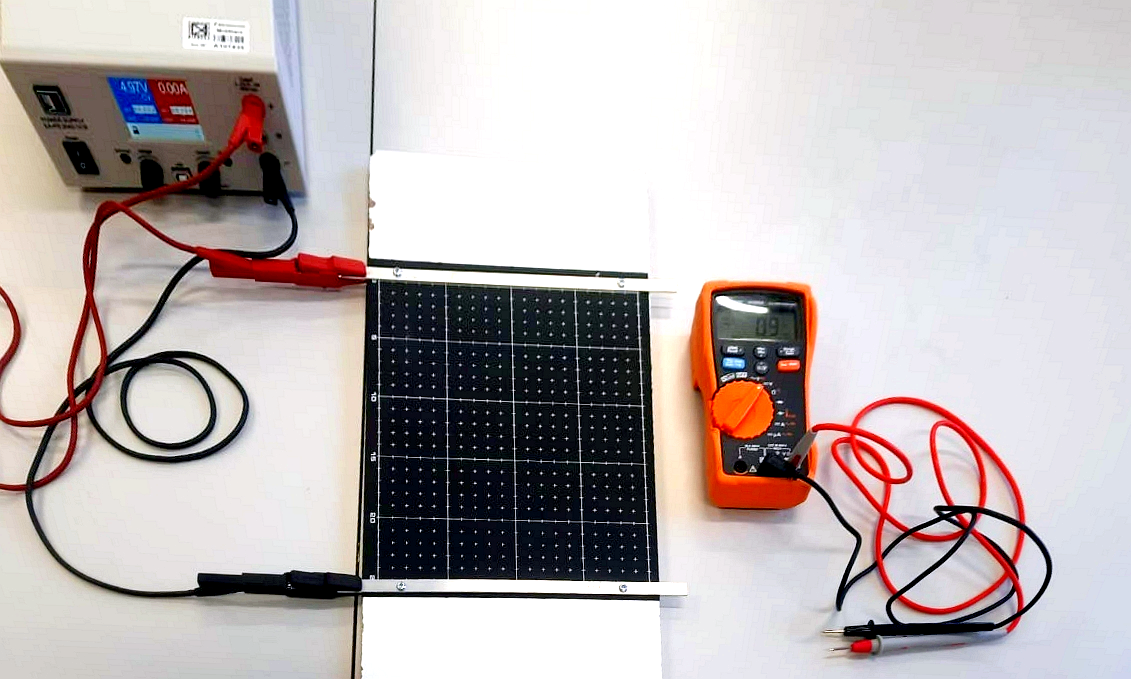
\includegraphics[width=\textwidth]{figures/visualize.png}};
    \begin{scope}[x={(image.south east)},y={(image.north west)}]
        \draw[->,red,ultra thick] (0.335,0.113) -- (0.335, 0.3); % Example arrow
        \draw[->,red,ultra thick] (0.32, 0.138) -- (0.44, 0.138); % Example arrow
        \node[align=center, text=red, font=\LARGE] at (0.41,0.17) {\(x\)}; % Example text
        \node[align=center, text=red, font=\LARGE] at (0.352,0.25) {\(y\)}; % Example text
    \end{scope}
\end{tikzpicture}
    \caption{Experimental setup for recording electric potential inside a
    conductor. In red are shown the axes used for addressing points.
The unit is the same as the smallest grid width on the
board, which marks centimeters. The origin \(0,0\) is placed at the intersection
of the axes }\label{fig:setup-visualize}
\end{figure}

\section{Analysis}
We analyzed the collected data to calculate the electric field at each point
restricted to the \(xy\) plane. The python script used to calculate and then
plot the field is shown in Listing~\ref{lst:script-1}. The script
achieves this by calculating at each point the difference quotients of the
potential with respect to \(x\) and \(y\) explicitly, this means:
\begin{align}
    E_x(x, y) = -\frac{\partial V}{\partial x} \approx -\frac{\Delta V}{\Delta
    x} = \frac{V_x{(x, y)} - V_x{(x+3, y)}}{3\,cm}\label{eq:diff-quotients_x}\\
    E_y(x, y) =  -\frac{\partial V}{\partial y} \approx -\frac{\Delta V}{\Delta
    y} = \frac{V_y{(x, y)} - V_y{(x, y+3)}}{3\,cm}\label{eq:diff-quotients_y}
\end{align}
where the 3 comes from how we sampled the points, which were 3 cm apart. 

\lstinputlisting[language=Python, caption={Python script for calculating the
electric field from the potential data},
label={lst:script-1}, firstline=1, lastline=8]{script.py}

Finally we plotted the electric vector field using the quiver plot function from
the matplotlib library. The resulting plot is shown in
\section{Results}
\section{Conclusion}
As we expected, the electric field lines are mostly vertical inside the board
and slightly curved on the edges. When modeling in a naive way the electric
field, we usually think of it completely vertical, as it would be in an infinite
parallel plate capacitor. However, in a real conductor, the field lines are more
curved on the edges, as we observed in the experiment. 

\chapter{Measuring the Earth’s Magnetic Field using a phone}

\section{Goal}
The main objective of our experiment is to determine the components of the Earth’s magnetic field. The principal components that we are talking about are: 
\begin{itemize}
    \item $B_h$, the horizontal component of the magnetic field;
    \item $B_v$, the vertical component of the magnetic field;
    \item $B$, the magnetic field;
    \item $\theta$, the angle between the horizontal and the vertical component.
\end{itemize}

\section{Method}
In order to achieve our goal, we performed the measurements using different tools:
\begin{itemize}
    \item A smartphone’s magnetometer and the Phyphox app;
    \item A rotating surface (chair), to better perform the rotation of the device;
    \item GPS Coordinates to determine geographic location;
    \item NOAA Magnetic Calculator to compute theoretical magnetic field values.
\end{itemize}

The last two tools were used to compare data with the ones that we collected in order to verify the reliability of the smartphone’s magnetometer. 

\section{Data and error analysis}
\subsection{Determine $B_h$}
In order to calculate the horizontal component of the magnetic field, we apply the following equation to our data: 
\[ B_h = \sqrt{B_x^2 + B_y^2} \]
where $B_x$ and $B_y$ are the magnetic field’s components along the x-axis and y-axis of the phone.

For the purpose of analyzing $B_h$, we have to determine $B_x$ and $B_y$ from the detected graphs on the Phyphox app. We downloaded the CSV file from the app, and thanks to Excel tools, we were able to estimate the specific values. Then inserting the values, we obtain our result: 
\[ B_h = \sqrt{20.62^2 + 11.25^2} = 21.62 \]

\subsection{Determine $B$}
In order to calculate $B$ (the magnetic field), combining $B_h$ (the horizontal component of the magnetic field) and $B_v$ (the vertical component), we have to apply the following formula:
\[ B = \sqrt{B_h^2 + B_v^2} \]
However, for the type of data that we used, $B_v$ is simply the mean of all the collected values of $B_z$ (the vertical component of the magnetic field along the z-axis of the phone). Obtaining that value, we calculate:
\[ B = \sqrt{21.62^2 + 60.18^2} = 64.42 \]

The formula that we used till now is the Pythagorean theorem viewed in a three-dimensional situation where, as we said before, $B_h$ is the horizontal component and $B_v$ is the average of the vertical component values.
$B$ is just the vector formed by combining the horizontal and vertical components of the magnetic field. Analyzing our results, we see a difference in the values of the total magnetic field and the horizontal component. This discrepancy represents the mutability of the Earth’s magnetic field being neither absolutely horizontal nor absolutely vertical but varying based on the geographical position.

\subsection{Determine $\theta$ and $B_v$}
In order to calculate the dip angle $\theta$, namely the angle between the horizontal component of $B$ ($B_h$) and $B$ itself, we have to derive it from a more general formula $B_h = B \cos(\theta)$.
From this and the data that we calculated in the previous points, we can extrapolate the angle:
\[ \theta = \arccos\left(\frac{B_h}{B}\right) = \arccos\left(\frac{21.62}{64.42}\right) = 70.39^\circ \]
Then, thanks to the angle that we found and the general formula stated before, we can calculate $B_v$:
\[ B_v = B \sin(\theta) = 64.42 \times \sin(70.39^\circ) = 60.68 \]

\subsection{Determine the amplitude of the signal}
The amplitude of the components of the Earth’s magnetic field is fundamental. With the app that we used, Phyphox, the recorded data could be analyzed directly on the device or exported as a CSV file for additional processing.
In order to calculate the specific amplitude, we have to sum, as we have done in the previous formula, all the amplitudes of the components along the x-, y-, z-axis:
\[ A = \sqrt{B_x^2 + B_y^2 + B_z^2} = 60.89 \]

\section{Conclusion}
In this experiment, we successfully measured the components of the Earth’s magnetic field, taking advantage of the help of a smartphone and the Phyphox app. All the results that we obtained for each component ($B_h$, $B_v$, $B$) matched our expectations.

All the data that we collected, however, were subject to errors caused by different elements:
\begin{itemize}
    \item Magnetic interference from nearby electronic devices or metallic objects;
    \item A non-constant rotation of the device due to human imprecision.
\end{itemize}

In the end, all the data were collected and analyzed correctly, giving us a precise and well-rounded analysis of Earth’s electromagnetic field.

\chapter{Measuring the Magnetic Field of a Coil}

\section{Goal}
The goal of this experiment is to determine the permeability of free space
(\(\mu_0\)) by measuring the magnetic field produced by a current-carrying coil.
This is achieved by varying the current intensity (\(I\)) and the number of
turns (\(N\)) of the coil, while keeping the distance (\(z\)) from the center of
the coil constant. The magnetic field strength (\(B\)) is measured using a
smartphone magnetometer.

\section{Method}
The experiment uses a circular coil of radius \(R = 7 \, \text{cm}\) with a
known number of loops (\(N\)). The magnetic field along the axis of the coil at
a distance \(z\) from its center is modeled by the equation:
\[
B(z) = \frac{\mu_0 N I R^2}{2 {\left(R^2 + z^2\right)}^{3/2}},
\]
where \(B(z)\) is the magnetic field at distance \(z\) (measured in
\(\mu\text{T}\)), \(\mu_0\) is permeability of free space (to be determined),
\(N\) number of loops in the coil, \(I\) the current through the coil (\(A\)),
\(R\) the radius of the coil  (\(m\)) and \(z\) the distance from the center of
the coil along its axis (\(m\)).


The experimental setups with different number of loops are shown in
figures~\ref{fig:magnetometer1} and~\ref{fig:magnetometer2}.
\begin{figure}
    \centering
    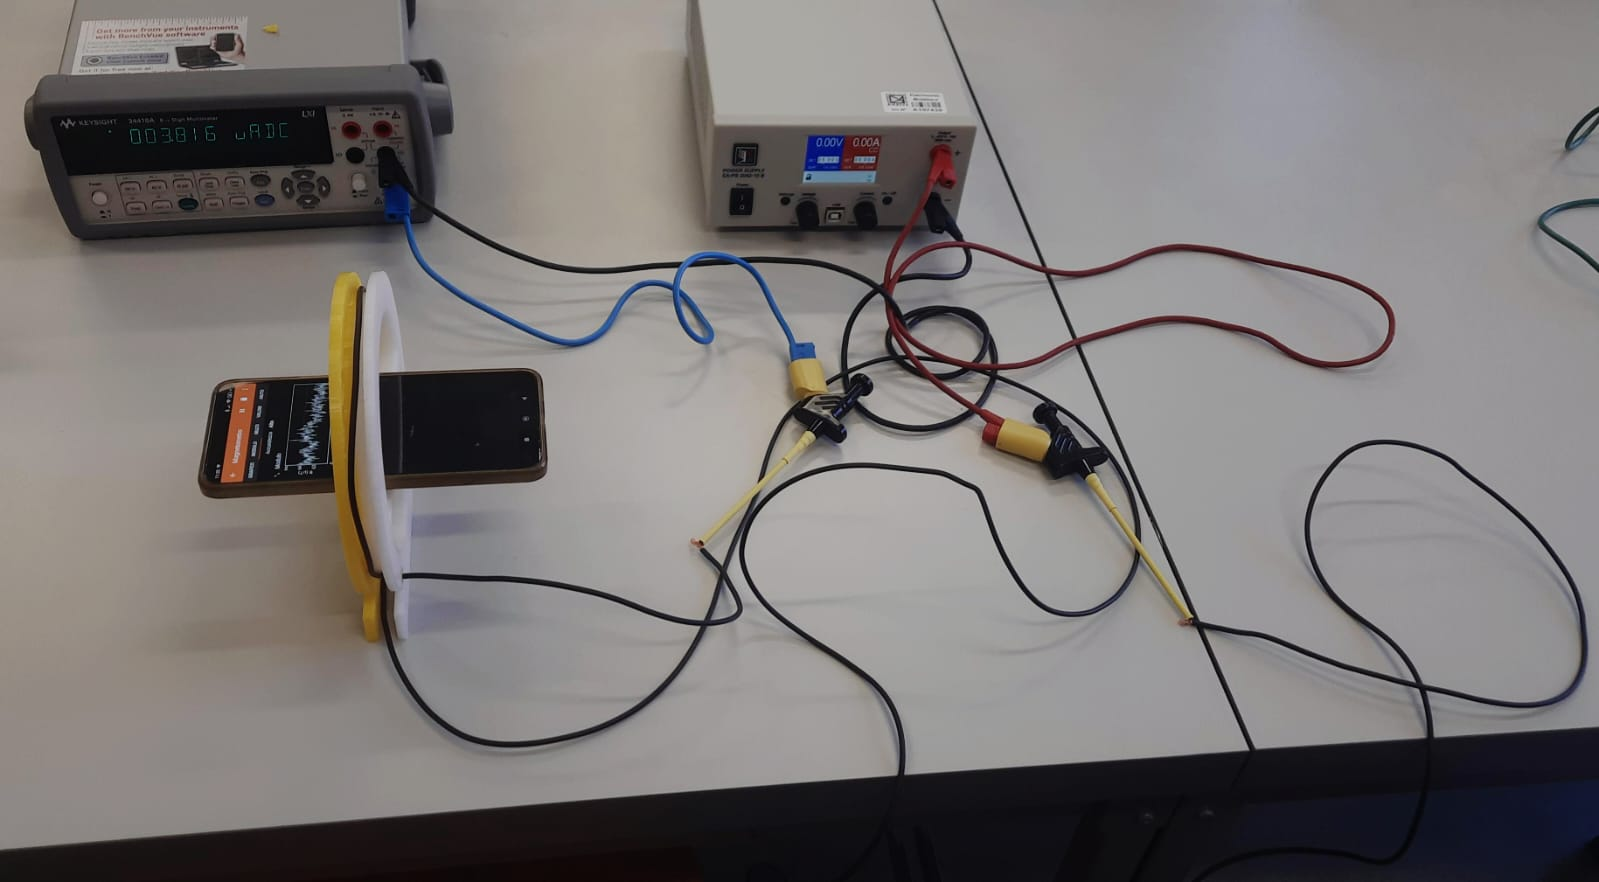
\includegraphics[width=0.5\linewidth]{figures/Magnetometer_1loop.jpeg}
    \caption{Magnetometer Setup with 1 Loop}\label{fig:magnetometer1}
\end{figure}
\begin{figure}
    \centering
    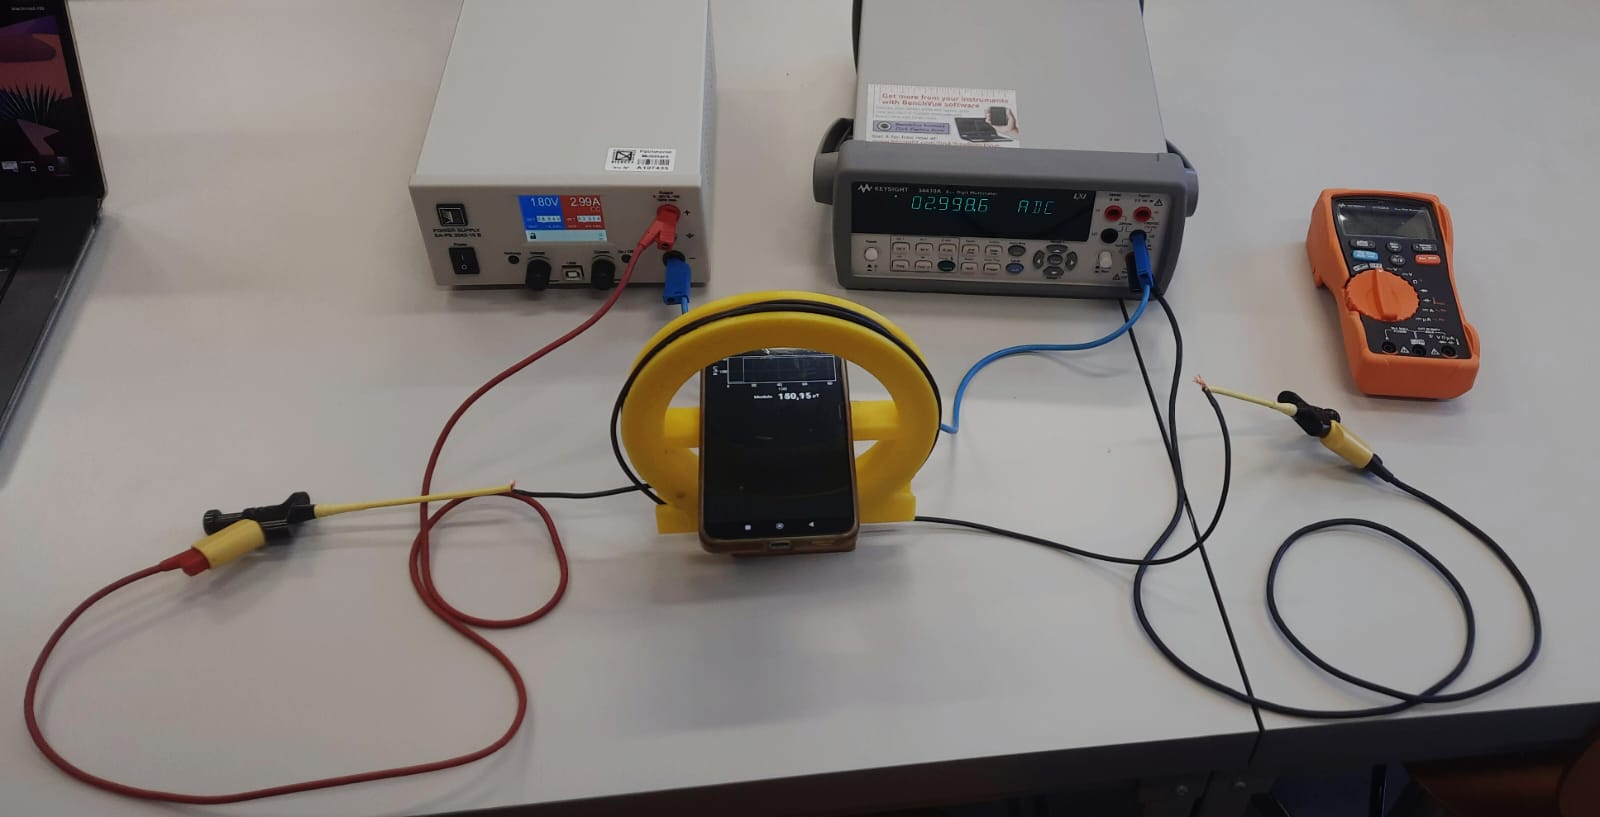
\includegraphics[width=0.5\linewidth]{figures/Magnetometer_multipleloops.jpeg}
    \caption{Magnetometer Setup with 10 Loops}\label{fig:magnetometer2}
\end{figure}

We used a coil wound on a plastic support, a current generator, a multimeter to measure current, and the Phyphox app on a smartphone to measure \(B\).

The magnetic field \(B\) was recorded for different values of \(I\) and \(N\), keeping \(z\) constant. The collected data was analyzed to calculate \(\mu_0\) by rearranging the formula for \(B(z)\).

\section{Data}
The data in table~\ref{tab:data} was collected during the experiment:

\begin{table}[h]
\centering
\begin{tabular}{cccc}
\toprule
Current (\(I\)) [A] & Turns (\(N\)) & Distance (\(z\)) [m] &
Avg. Abs. Field          (\(B\)) [\(\mu\text{T}\)]\\
\midrule
0.000006& 1& 0.06& 0.00003\\
2.0 & 5& 0.06& 34.5\\
3.0 & 5& 0.06& 62.2\\
0.000006& 10& 0.06& 0.0004\\
2.0 & 10& 0.06& 78.7\\
3.0 & 10& 0.06& 118.2\\
\bottomrule
\end{tabular}
\caption{Collected data showing magnetic field measurements at different
currents and coil configurations.}\label{tab:data}
\end{table}
The Absolute Magnetic Field (\(B\)) [\(\mu\text{T}\)] is the magnitude of the magnetic field vector, calculated using the formula:

\[
B = \sqrt{B_x^2 + B_y^2 + B_z^2}
\]
It is calculated using all three (x, y and z) coordinates recorded in the
Phyphox app. In the table~\ref{tab:data} we calculated the averages of
Absolute Magnetic Fields for each row using the Excel data from the Phyphox
magnetometer.

We found the distance (\(z\)) value is \(4 \, \text{cm}\) by using a ruler to
measure the axial distance from the center of the coil to the point where the
magnetic field is being measured.  

\section{Analysis}
We rearrange the formula to compute \(\mu_0\):
\[
    \mu_0 = \frac{2 B(z) {\left(R^2 + z^2\right)}^{3/2}}{N I R^2}.
\]
Calculate the average and standard deviation of \(\mu_0\) across all
measurements to account for experimental variability. Compare the experimental
value of \(\mu_0\) with the theoretical value of \(4\pi \times 10^{-7} \,
\text{T·m/A}\).


\subsection{Results}

\begin{lstlisting}[language=Python, caption={Python code for calculating \(\mu_0\)}, basicstyle=\ttfamily\footnotesize, keywordstyle=\color{blue}, commentstyle=\color{gray}]
import numpy as np

# Constants
R = 0.07  # Radius of the coil (in meters)
mu_0_theoretical = 4 * np.pi * 1e-7  # Theoretical value of mu_0 in Tm/A

# Data (Current, Number of Turns, Distance, Magnetic Field)
data = [
    (0.000006, 1, 0.06, 0.00003),
    (2.0, 5, 0.06, 34.5),
    (3.0, 5, 0.06, 62.2),
    (0.000006, 10, 0.06, 0.0004),
    (2.0, 10, 0.06, 78.7),
    (3.0, 10, 0.06, 118.2)
]

# Function to calculate mu_0 from the formula
def calculate_mu_0(B, N, I, z, R):
    return (2 * B * (R**2 + z**2)**(3/2)) / (N * I * R**2)

# Calculate mu_0 for each measurement
mu_0_values = []
for I, N, z, B in data:
    mu_0 = calculate_mu_0(B * 1e-6, N, I, z, R)  # Convert B to Tesla (since B is in microteslas)
    mu_0_values.append(mu_0)

# Calculate the average and standard deviation of mu_0
mu_0_average = np.mean(mu_0_values)
mu_0_std_dev = np.std(mu_0_values)

# Output the results
print(f"Average mu_0: {mu_0_average:.5e} Tm/A")
print(f"Standard deviation of mu_0: {mu_0_std_dev:.5e} Tm/A")
print(f"Theoretical mu_0: {mu_0_theoretical:.5e} Tm/A")
\end{lstlisting}

The computed values of magnetic permeability \(\mu_0\) are as follows:

Average value of \(\mu_0\): 
    \[
    \mu_0 \approx 1.4569 \times 10^{-6} \, \text{T·m/A}
    \]
    
Standard deviation of \(\mu_0\): 
    \[
    \sigma_{\mu_0} \approx 3.281 \times 10^{-7} \, \text{T·m/A}
    \]
    
Theoretical value of \(\mu_0\): 
    \[
    \mu_0^{\text{theoretical}} = 1.257 \times 10^{-6} \, \text{T·m/A}
    \]
The experimental results are in reasonable agreement with the theoretical value of \(\mu_0\). The difference is within the experimental uncertainty, as indicated by the standard deviation. While the experimental value is slightly higher than the theoretical value, this discrepancy is small enough to be considered within the expected experimental error, especially in light of the standard deviation. 


\end{document}


